\documentclass[1p]{elsarticle_modified}
%\bibliographystyle{elsarticle-num}

%\usepackage[colorlinks]{hyperref}
%\usepackage{abbrmath_seonhwa} %\Abb, \Ascr, \Acal ,\Abf, \Afrak
\usepackage{amsfonts}
\usepackage{amssymb}
\usepackage{amsmath}
\usepackage{amsthm}
\usepackage{scalefnt}
\usepackage{amsbsy}
\usepackage{kotex}
\usepackage{caption}
\usepackage{subfig}
\usepackage{color}
\usepackage{graphicx}
\usepackage{xcolor} %% white, black, red, green, blue, cyan, magenta, yellow
\usepackage{float}
\usepackage{setspace}
\usepackage{hyperref}

\usepackage{tikz}
\usetikzlibrary{arrows}

\usepackage{multirow}
\usepackage{array} % fixed length table
\usepackage{hhline}

%%%%%%%%%%%%%%%%%%%%%
\makeatletter
\renewcommand*\env@matrix[1][\arraystretch]{%
	\edef\arraystretch{#1}%
	\hskip -\arraycolsep
	\let\@ifnextchar\new@ifnextchar
	\array{*\c@MaxMatrixCols c}}
\makeatother %https://tex.stackexchange.com/questions/14071/how-can-i-increase-the-line-spacing-in-a-matrix
%%%%%%%%%%%%%%%

\usepackage[normalem]{ulem}

\newcommand{\msout}[1]{\ifmmode\text{\sout{\ensuremath{#1}}}\else\sout{#1}\fi}
%SOURCE: \msout is \stkout macro in https://tex.stackexchange.com/questions/20609/strikeout-in-math-mode

\newcommand{\cancel}[1]{
	\ifmmode
	{\color{red}\msout{#1}}
	\else
	{\color{red}\sout{#1}}
	\fi
}

\newcommand{\add}[1]{
	{\color{blue}\uwave{#1}}
}

\newcommand{\replace}[2]{
	\ifmmode
	{\color{red}\msout{#1}}{\color{blue}\uwave{#2}}
	\else
	{\color{red}\sout{#1}}{\color{blue}\uwave{#2}}
	\fi
}

\newcommand{\Sol}{\mathcal{S}} %segment
\newcommand{\D}{D} %diagram
\newcommand{\A}{\mathcal{A}} %arc


%%%%%%%%%%%%%%%%%%%%%%%%%%%%%5 test

\def\sl{\operatorname{\textup{SL}}(2,\Cbb)}
\def\psl{\operatorname{\textup{PSL}}(2,\Cbb)}
\def\quan{\mkern 1mu \triangleright \mkern 1mu}

\theoremstyle{definition}
\newtheorem{thm}{Theorem}[section]
\newtheorem{prop}[thm]{Proposition}
\newtheorem{lem}[thm]{Lemma}
\newtheorem{ques}[thm]{Question}
\newtheorem{cor}[thm]{Corollary}
\newtheorem{defn}[thm]{Definition}
\newtheorem{exam}[thm]{Example}
\newtheorem{rmk}[thm]{Remark}
\newtheorem{alg}[thm]{Algorithm}

\newcommand{\I}{\sqrt{-1}}
\begin{document}

%\begin{frontmatter}
%
%\title{Boundary parabolic representations of knots up to 8 crossings}
%
%%% Group authors per affiliation:
%\author{Yunhi Cho} 
%\address{Department of Mathematics, University of Seoul, Seoul, Korea}
%\ead{yhcho@uos.ac.kr}
%
%
%\author{Seonhwa Kim} %\fnref{s_kim}}
%\address{Center for Geometry and Physics, Institute for Basic Science, Pohang, 37673, Korea}
%\ead{ryeona17@ibs.re.kr}
%
%\author{Hyuk Kim}
%\address{Department of Mathematical Sciences, Seoul National University, Seoul 08826, Korea}
%\ead{hyukkim@snu.ac.kr}
%
%\author{Seokbeom Yoon}
%\address{Department of Mathematical Sciences, Seoul National University, Seoul, 08826,  Korea}
%\ead{sbyoon15@snu.ac.kr}
%
%\begin{abstract}
%We find all boundary parabolic representation of knots up to 8 crossings.
%
%\end{abstract}
%\begin{keyword}
%    \MSC[2010] 57M25 
%\end{keyword}
%
%\end{frontmatter}

%\linenumbers
%\tableofcontents
%
\newcommand\colored[1]{\textcolor{white}{\rule[-0.35ex]{0.8em}{1.4ex}}\kern-0.8em\color{red} #1}%
%\newcommand\colored[1]{\textcolor{white}{ #1}\kern-2.17ex	\textcolor{white}{ #1}\kern-1.81ex	\textcolor{white}{ #1}\kern-2.15ex\color{red}#1	}

{\Large $\underline{12a_{0160}~(K12a_{0160})}$}

\setlength{\tabcolsep}{10pt}
\renewcommand{\arraystretch}{1.6}
\vspace{1cm}\begin{tabular}{m{100pt}>{\centering\arraybackslash}m{274pt}}
\multirow{5}{120pt}{
	\centering
	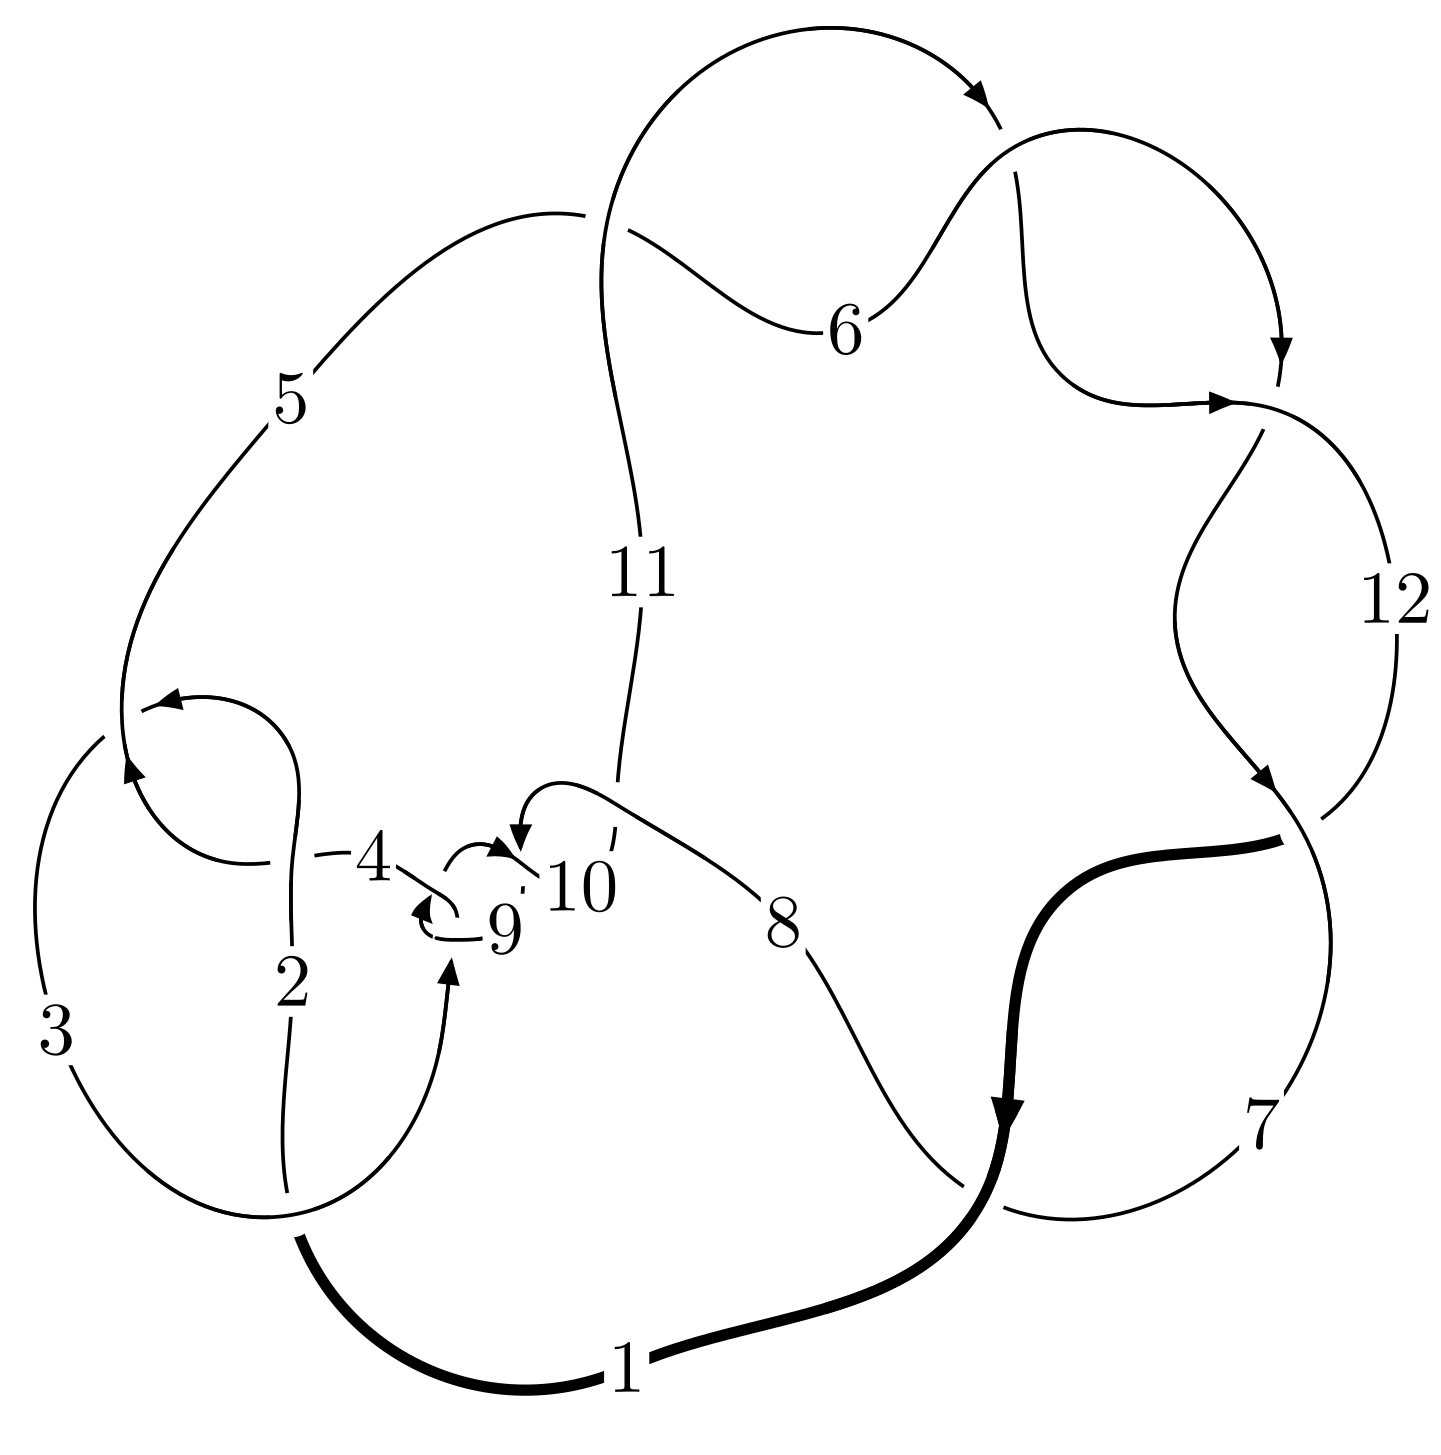
\includegraphics[width=112pt]{../../../GIT/diagram.site/Diagrams/png/961_12a_0160.png}\\
\ \ \ A knot diagram\footnotemark}&
\allowdisplaybreaks
\textbf{Linearized knot diagam} \\
\cline{2-2}
 &
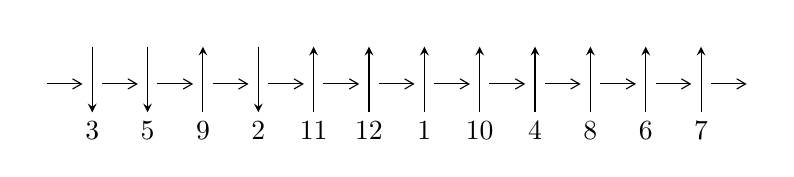
\begin{tikzpicture}[x=20pt, y=17pt]
	% nodes
	\node (C0) at (0, 0) {};
	\node (C1) at (1, 0) {};
	\node (C1U) at (1, +1) {};
	\node (C1D) at (1, -1) {3};

	\node (C2) at (2, 0) {};
	\node (C2U) at (2, +1) {};
	\node (C2D) at (2, -1) {5};

	\node (C3) at (3, 0) {};
	\node (C3U) at (3, +1) {};
	\node (C3D) at (3, -1) {9};

	\node (C4) at (4, 0) {};
	\node (C4U) at (4, +1) {};
	\node (C4D) at (4, -1) {2};

	\node (C5) at (5, 0) {};
	\node (C5U) at (5, +1) {};
	\node (C5D) at (5, -1) {11};

	\node (C6) at (6, 0) {};
	\node (C6U) at (6, +1) {};
	\node (C6D) at (6, -1) {12};

	\node (C7) at (7, 0) {};
	\node (C7U) at (7, +1) {};
	\node (C7D) at (7, -1) {1};

	\node (C8) at (8, 0) {};
	\node (C8U) at (8, +1) {};
	\node (C8D) at (8, -1) {10};

	\node (C9) at (9, 0) {};
	\node (C9U) at (9, +1) {};
	\node (C9D) at (9, -1) {4};

	\node (C10) at (10, 0) {};
	\node (C10U) at (10, +1) {};
	\node (C10D) at (10, -1) {8};

	\node (C11) at (11, 0) {};
	\node (C11U) at (11, +1) {};
	\node (C11D) at (11, -1) {6};

	\node (C12) at (12, 0) {};
	\node (C12U) at (12, +1) {};
	\node (C12D) at (12, -1) {7};
	\node (C13) at (13, 0) {};

	% arrows
	\draw[->,>={angle 60}]
	(C0) edge (C1) (C1) edge (C2) (C2) edge (C3) (C3) edge (C4) (C4) edge (C5) (C5) edge (C6) (C6) edge (C7) (C7) edge (C8) (C8) edge (C9) (C9) edge (C10) (C10) edge (C11) (C11) edge (C12) (C12) edge (C13) ;	\draw[->,>=stealth]
	(C1U) edge (C1D) (C2U) edge (C2D) (C3D) edge (C3U) (C4U) edge (C4D) (C5D) edge (C5U) (C6D) edge (C6U) (C7D) edge (C7U) (C8D) edge (C8U) (C9D) edge (C9U) (C10D) edge (C10U) (C11D) edge (C11U) (C12D) edge (C12U) ;
	\end{tikzpicture} \\
\hhline{~~} \\& 
\textbf{Solving Sequence} \\ \cline{2-2} 
 &
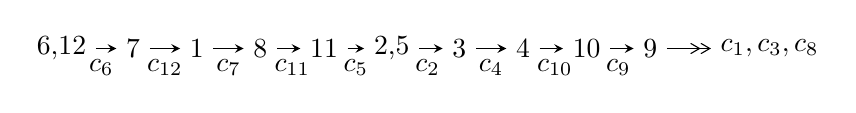
\begin{tikzpicture}[x=23pt, y=7pt]
	% node
	\node (A0) at (-1/8, 0) {6,12};
	\node (A1) at (1, 0) {7};
	\node (A2) at (2, 0) {1};
	\node (A3) at (3, 0) {8};
	\node (A4) at (4, 0) {11};
	\node (A5) at (81/16, 0) {2,5};
	\node (A6) at (49/8, 0) {3};
	\node (A7) at (57/8, 0) {4};
	\node (A8) at (65/8, 0) {10};
	\node (A9) at (73/8, 0) {9};
	\node (C1) at (1/2, -1) {$c_{6}$};
	\node (C2) at (3/2, -1) {$c_{12}$};
	\node (C3) at (5/2, -1) {$c_{7}$};
	\node (C4) at (7/2, -1) {$c_{11}$};
	\node (C5) at (9/2, -1) {$c_{5}$};
	\node (C6) at (45/8, -1) {$c_{2}$};
	\node (C7) at (53/8, -1) {$c_{4}$};
	\node (C8) at (61/8, -1) {$c_{10}$};
	\node (C9) at (69/8, -1) {$c_{9}$};
	\node (A10) at (11, 0) {$c_{1},c_{3},c_{8}$};

	% edge
	\draw[->,>=stealth]	
	(A0) edge (A1) (A1) edge (A2) (A2) edge (A3) (A3) edge (A4) (A4) edge (A5) (A5) edge (A6) (A6) edge (A7) (A7) edge (A8) (A8) edge (A9) ;
	\draw[->>,>={angle 60}]	
	(A9) edge (A10);
\end{tikzpicture} \\ 

\end{tabular} \\

\footnotetext{
The image of knot diagram is generated by the software ``\textbf{Draw programme}" developed by Andrew Bartholomew(\url{http://www.layer8.co.uk/maths/draw/index.htm\#Running-draw}), where we modified some parts for our purpose(\url{https://github.com/CATsTAILs/LinksPainter}).
}\phantom \\ \newline 
\centering \textbf{Ideals for irreducible components\footnotemark of $X_{\text{par}}$} 
 
\begin{align*}
I^u_{1}&=\langle 
u^{51}+u^{50}+\cdots+b- u,\;- u^{51}- u^{50}+\cdots+a-1,\;u^{52}+2 u^{51}+\cdots+2 u+1\rangle \\
I^u_{2}&=\langle 
b+u+2,\;a- u-1,\;u^2- u-1\rangle \\
\\
\end{align*}
\raggedright * 2 irreducible components of $\dim_{\mathbb{C}}=0$, with total 54 representations.\\
\footnotetext{All coefficients of polynomials are rational numbers. But the coefficients are sometimes approximated in decimal forms when there is not enough margin.}
\newpage
\renewcommand{\arraystretch}{1}
\centering \section*{I. $I^u_{1}= \langle u^{51}+u^{50}+\cdots+b- u,\;- u^{51}- u^{50}+\cdots+a-1,\;u^{52}+2 u^{51}+\cdots+2 u+1 \rangle$}
\flushleft \textbf{(i) Arc colorings}\\
\begin{tabular}{m{7pt} m{180pt} m{7pt} m{180pt} }
\flushright $a_{6}=$&$\begin{pmatrix}1\\0\end{pmatrix}$ \\
\flushright $a_{12}=$&$\begin{pmatrix}0\\u\end{pmatrix}$ \\
\flushright $a_{7}=$&$\begin{pmatrix}1\\- u^2\end{pmatrix}$ \\
\flushright $a_{1}=$&$\begin{pmatrix}u\\- u^3+u\end{pmatrix}$ \\
\flushright $a_{8}=$&$\begin{pmatrix}- u^2+1\\u^4-2 u^2\end{pmatrix}$ \\
\flushright $a_{11}=$&$\begin{pmatrix}- u\\u\end{pmatrix}$ \\
\flushright $a_{2}=$&$\begin{pmatrix}u^{51}+u^{50}+\cdots+7 u+1\\- u^{51}- u^{50}+\cdots-4 u^2+u\end{pmatrix}$ \\
\flushright $a_{5}=$&$\begin{pmatrix}- u^2+1\\u^2\end{pmatrix}$ \\
\flushright $a_{3}=$&$\begin{pmatrix}u^{50}+u^{49}+\cdots+18 u^2+5 u\\u^{51}-32 u^{49}+\cdots+2 u+1\end{pmatrix}$ \\
\flushright $a_{4}=$&$\begin{pmatrix}-2 u^{51}- u^{50}+\cdots-7 u-1\\3 u^{51}+2 u^{50}+\cdots+u+1\end{pmatrix}$ \\
\flushright $a_{10}=$&$\begin{pmatrix}u^7-4 u^5+4 u^3-2 u\\- u^9+5 u^7-7 u^5+2 u^3+u\end{pmatrix}$ \\
\flushright $a_{9}=$&$\begin{pmatrix}- u^{12}+7 u^{10}-17 u^8+18 u^6-10 u^4+u^2+1\\u^{14}-8 u^{12}+23 u^{10}-28 u^8+12 u^6+2 u^4-3 u^2\end{pmatrix}$\\&\end{tabular}
\flushleft \textbf{(ii) Obstruction class $= -1$}\\~\\
\flushleft \textbf{(iii) Cusp Shapes $= 8 u^{51}+9 u^{50}+\cdots-9 u+11$}\\~\\
\newpage\renewcommand{\arraystretch}{1}
\flushleft \textbf{(iv) u-Polynomials at the component}\newline \\
\begin{tabular}{m{50pt}|m{274pt}}
Crossings & \hspace{64pt}u-Polynomials at each crossing \\
\hline $$\begin{aligned}c_{1}\end{aligned}$$&$\begin{aligned}
&u^{52}+29 u^{51}+\cdots+29 u+1
\end{aligned}$\\
\hline $$\begin{aligned}c_{2},c_{4}\end{aligned}$$&$\begin{aligned}
&u^{52}-3 u^{51}+\cdots-9 u+1
\end{aligned}$\\
\hline $$\begin{aligned}c_{3},c_{9}\end{aligned}$$&$\begin{aligned}
&u^{52}- u^{51}+\cdots-4 u+4
\end{aligned}$\\
\hline $$\begin{aligned}c_{5},c_{6},c_{7}\\c_{11},c_{12}\end{aligned}$$&$\begin{aligned}
&u^{52}-2 u^{51}+\cdots-2 u+1
\end{aligned}$\\
\hline $$\begin{aligned}c_{8},c_{10}\end{aligned}$$&$\begin{aligned}
&u^{52}-15 u^{51}+\cdots-248 u+16
\end{aligned}$\\
\hline
\end{tabular}\\~\\
\newpage\renewcommand{\arraystretch}{1}
\flushleft \textbf{(v) Riley Polynomials at the component}\newline \\
\begin{tabular}{m{50pt}|m{274pt}}
Crossings & \hspace{64pt}Riley Polynomials at each crossing \\
\hline $$\begin{aligned}c_{1}\end{aligned}$$&$\begin{aligned}
&y^{52}-9 y^{51}+\cdots-593 y+1
\end{aligned}$\\
\hline $$\begin{aligned}c_{2},c_{4}\end{aligned}$$&$\begin{aligned}
&y^{52}-29 y^{51}+\cdots-29 y+1
\end{aligned}$\\
\hline $$\begin{aligned}c_{3},c_{9}\end{aligned}$$&$\begin{aligned}
&y^{52}-15 y^{51}+\cdots-248 y+16
\end{aligned}$\\
\hline $$\begin{aligned}c_{5},c_{6},c_{7}\\c_{11},c_{12}\end{aligned}$$&$\begin{aligned}
&y^{52}-66 y^{51}+\cdots+6 y+1
\end{aligned}$\\
\hline $$\begin{aligned}c_{8},c_{10}\end{aligned}$$&$\begin{aligned}
&y^{52}+41 y^{51}+\cdots-9504 y+256
\end{aligned}$\\
\hline
\end{tabular}\\~\\
\newpage\flushleft \textbf{(vi) Complex Volumes and Cusp Shapes}
$$\begin{array}{c|c|c}  
\text{Solutions to }I^u_{1}& \I (\text{vol} + \sqrt{-1}CS) & \text{Cusp shape}\\
 \hline 
\begin{aligned}
u &= \phantom{-}1.002200 + 0.101685 I \\
a &= \phantom{-}0.620325 + 0.568001 I \\
b &= -0.338736 - 0.201694 I\end{aligned}
 & \phantom{-}5.42587 + 0.91536 I & \phantom{-}15.8250 + 0. I\phantom{ +0.000000I} \\ \hline\begin{aligned}
u &= \phantom{-}1.002200 - 0.101685 I \\
a &= \phantom{-}0.620325 - 0.568001 I \\
b &= -0.338736 + 0.201694 I\end{aligned}
 & \phantom{-}5.42587 - 0.91536 I & \phantom{-}15.8250 + 0. I\phantom{ +0.000000I} \\ \hline\begin{aligned}
u &= \phantom{-}0.900408 + 0.415514 I \\
a &= -0.686316 + 0.426160 I \\
b &= -1.32817 - 1.98079 I\end{aligned}
 & -2.89703 + 10.97490 I & \phantom{-}6.84879 - 9.10557 I \\ \hline\begin{aligned}
u &= \phantom{-}0.900408 - 0.415514 I \\
a &= -0.686316 - 0.426160 I \\
b &= -1.32817 + 1.98079 I\end{aligned}
 & -2.89703 - 10.97490 I & \phantom{-}6.84879 + 9.10557 I \\ \hline\begin{aligned}
u &= \phantom{-}0.993272 + 0.210152 I \\
a &= \phantom{-}0.306112 - 0.310737 I \\
b &= -1.09437 - 1.05834 I\end{aligned}
 & \phantom{-}4.36145 + 5.53576 I & \phantom{-}12.8247 - 7.7042 I \\ \hline\begin{aligned}
u &= \phantom{-}0.993272 - 0.210152 I \\
a &= \phantom{-}0.306112 + 0.310737 I \\
b &= -1.09437 + 1.05834 I\end{aligned}
 & \phantom{-}4.36145 - 5.53576 I & \phantom{-}12.8247 + 7.7042 I \\ \hline\begin{aligned}
u &= \phantom{-}0.887221 + 0.376671 I \\
a &= \phantom{-}0.216936 + 0.254530 I \\
b &= \phantom{-}0.512607 - 0.524064 I\end{aligned}
 & \phantom{-}0.28073 + 6.02352 I & \phantom{-}10.12786 - 6.24694 I \\ \hline\begin{aligned}
u &= \phantom{-}0.887221 - 0.376671 I \\
a &= \phantom{-}0.216936 - 0.254530 I \\
b &= \phantom{-}0.512607 + 0.524064 I\end{aligned}
 & \phantom{-}0.28073 - 6.02352 I & \phantom{-}10.12786 + 6.24694 I \\ \hline\begin{aligned}
u &= -0.853207 + 0.384206 I \\
a &= \phantom{-}0.903606 + 0.104965 I \\
b &= \phantom{-}1.14253 - 1.97773 I\end{aligned}
 & -3.75080 - 4.74137 I & \phantom{-}5.53664 + 4.96484 I \\ \hline\begin{aligned}
u &= -0.853207 - 0.384206 I \\
a &= \phantom{-}0.903606 - 0.104965 I \\
b &= \phantom{-}1.14253 + 1.97773 I\end{aligned}
 & -3.75080 + 4.74137 I & \phantom{-}5.53664 - 4.96484 I\\
 \hline 
 \end{array}$$\newpage$$\begin{array}{c|c|c}  
\text{Solutions to }I^u_{1}& \I (\text{vol} + \sqrt{-1}CS) & \text{Cusp shape}\\
 \hline 
\begin{aligned}
u &= \phantom{-}0.825680 + 0.382316 I \\
a &= -0.111743 - 0.969230 I \\
b &= \phantom{-}1.57224 + 1.67207 I\end{aligned}
 & -3.92292 + 1.91465 I & \phantom{-}5.33907 - 3.86780 I \\ \hline\begin{aligned}
u &= \phantom{-}0.825680 - 0.382316 I \\
a &= -0.111743 + 0.969230 I \\
b &= \phantom{-}1.57224 - 1.67207 I\end{aligned}
 & -3.92292 - 1.91465 I & \phantom{-}5.33907 + 3.86780 I \\ \hline\begin{aligned}
u &= -0.768059 + 0.439344 I \\
a &= -0.195399 - 0.893583 I \\
b &= -1.17619 + 1.70576 I\end{aligned}
 & -3.69972 + 3.78870 I & \phantom{-}5.61035 - 2.00055 I \\ \hline\begin{aligned}
u &= -0.768059 - 0.439344 I \\
a &= -0.195399 + 0.893583 I \\
b &= -1.17619 - 1.70576 I\end{aligned}
 & -3.69972 - 3.78870 I & \phantom{-}5.61035 + 2.00055 I \\ \hline\begin{aligned}
u &= -0.869138 + 0.090566 I \\
a &= -0.624942 - 0.906814 I \\
b &= \phantom{-}0.124670 - 0.964759 I\end{aligned}
 & \phantom{-}1.28982 - 1.61982 I & \phantom{-}10.04112 + 4.38556 I \\ \hline\begin{aligned}
u &= -0.869138 - 0.090566 I \\
a &= -0.624942 + 0.906814 I \\
b &= \phantom{-}0.124670 + 0.964759 I\end{aligned}
 & \phantom{-}1.28982 + 1.61982 I & \phantom{-}10.04112 - 4.38556 I \\ \hline\begin{aligned}
u &= -0.778648 + 0.361263 I \\
a &= -0.381137 + 0.106397 I \\
b &= -0.541900 - 0.279638 I\end{aligned}
 & -0.394378 - 0.492969 I & \phantom{-}9.04055 + 1.45710 I \\ \hline\begin{aligned}
u &= -0.778648 - 0.361263 I \\
a &= -0.381137 - 0.106397 I \\
b &= -0.541900 + 0.279638 I\end{aligned}
 & -0.394378 + 0.492969 I & \phantom{-}9.04055 - 1.45710 I \\ \hline\begin{aligned}
u &= \phantom{-}0.803120\phantom{ +0.000000I} \\
a &= -0.675162\phantom{ +0.000000I} \\
b &= \phantom{-}2.05557\phantom{ +0.000000I}\end{aligned}
 & \phantom{-}0.0369555\phantom{ +0.000000I} & \phantom{-}14.8580\phantom{ +0.000000I} \\ \hline\begin{aligned}
u &= -0.062250 + 0.639708 I \\
a &= -3.04229 + 0.33326 I \\
b &= \phantom{-}0.028753 - 0.273837 I\end{aligned}
 & -5.82794 - 7.41916 I & \phantom{-}2.02402 + 6.23213 I\\
 \hline 
 \end{array}$$\newpage$$\begin{array}{c|c|c}  
\text{Solutions to }I^u_{1}& \I (\text{vol} + \sqrt{-1}CS) & \text{Cusp shape}\\
 \hline 
\begin{aligned}
u &= -0.062250 - 0.639708 I \\
a &= -3.04229 - 0.33326 I \\
b &= \phantom{-}0.028753 + 0.273837 I\end{aligned}
 & -5.82794 + 7.41916 I & \phantom{-}2.02402 - 6.23213 I \\ \hline\begin{aligned}
u &= \phantom{-}0.013286 + 0.599769 I \\
a &= \phantom{-}3.16045 + 0.60539 I \\
b &= \phantom{-}0.050264 - 0.426280 I\end{aligned}
 & -6.37556 + 1.41175 I & \phantom{-}0.512224 - 0.772694 I \\ \hline\begin{aligned}
u &= \phantom{-}0.013286 - 0.599769 I \\
a &= \phantom{-}3.16045 - 0.60539 I \\
b &= \phantom{-}0.050264 + 0.426280 I\end{aligned}
 & -6.37556 - 1.41175 I & \phantom{-}0.512224 + 0.772694 I \\ \hline\begin{aligned}
u &= -0.051648 + 0.589699 I \\
a &= -0.118187 + 0.761845 I \\
b &= \phantom{-}0.019107 + 0.393978 I\end{aligned}
 & -2.57484 - 2.75018 I & \phantom{-}4.73313 + 3.20106 I \\ \hline\begin{aligned}
u &= -0.051648 - 0.589699 I \\
a &= -0.118187 - 0.761845 I \\
b &= \phantom{-}0.019107 - 0.393978 I\end{aligned}
 & -2.57484 + 2.75018 I & \phantom{-}4.73313 - 3.20106 I \\ \hline\begin{aligned}
u &= -0.429505 + 0.363992 I \\
a &= -0.283846 + 0.092161 I \\
b &= -0.501430 + 0.658806 I\end{aligned}
 & \phantom{-}0.985801 + 0.373941 I & \phantom{-}10.64681 + 0.40187 I \\ \hline\begin{aligned}
u &= -0.429505 - 0.363992 I \\
a &= -0.283846 - 0.092161 I \\
b &= -0.501430 - 0.658806 I\end{aligned}
 & \phantom{-}0.985801 - 0.373941 I & \phantom{-}10.64681 - 0.40187 I \\ \hline\begin{aligned}
u &= -0.260485 + 0.467225 I \\
a &= -1.65751 + 0.54880 I \\
b &= -0.417669 - 0.022465 I\end{aligned}
 & \phantom{-}0.44749 - 3.27943 I & \phantom{-}7.33672 + 8.28421 I \\ \hline\begin{aligned}
u &= -0.260485 - 0.467225 I \\
a &= -1.65751 - 0.54880 I \\
b &= -0.417669 + 0.022465 I\end{aligned}
 & \phantom{-}0.44749 + 3.27943 I & \phantom{-}7.33672 - 8.28421 I \\ \hline\begin{aligned}
u &= -0.449135\phantom{ +0.000000I} \\
a &= -0.461577\phantom{ +0.000000I} \\
b &= -0.372331\phantom{ +0.000000I}\end{aligned}
 & \phantom{-}0.706606\phantom{ +0.000000I} & \phantom{-}14.1070\phantom{ +0.000000I}\\
 \hline 
 \end{array}$$\newpage$$\begin{array}{c|c|c}  
\text{Solutions to }I^u_{1}& \I (\text{vol} + \sqrt{-1}CS) & \text{Cusp shape}\\
 \hline 
\begin{aligned}
u &= \phantom{-}1.58988\phantom{ +0.000000I} \\
a &= \phantom{-}2.20327\phantom{ +0.000000I} \\
b &= -3.13699\phantom{ +0.000000I}\end{aligned}
 & \phantom{-}7.80979\phantom{ +0.000000I} & \phantom{-0.000000 } 0 \\ \hline\begin{aligned}
u &= \phantom{-}1.62815 + 0.10007 I \\
a &= \phantom{-}2.77026 + 1.09581 I \\
b &= -3.78872 - 1.31091 I\end{aligned}
 & \phantom{-}4.49371 - 1.83490 I & \phantom{-0.000000 } 0 \\ \hline\begin{aligned}
u &= \phantom{-}1.62815 - 0.10007 I \\
a &= \phantom{-}2.77026 - 1.09581 I \\
b &= -3.78872 + 1.31091 I\end{aligned}
 & \phantom{-}4.49371 + 1.83490 I & \phantom{-0.000000 } 0 \\ \hline\begin{aligned}
u &= \phantom{-}1.65492 + 0.07803 I \\
a &= \phantom{-}0.986803 - 0.272171 I \\
b &= -1.64509 + 0.11104 I\end{aligned}
 & \phantom{-}8.08427 + 2.03863 I & \phantom{-0.000000 } 0 \\ \hline\begin{aligned}
u &= \phantom{-}1.65492 - 0.07803 I \\
a &= \phantom{-}0.986803 + 0.272171 I \\
b &= -1.64509 - 0.11104 I\end{aligned}
 & \phantom{-}8.08427 - 2.03863 I & \phantom{-0.000000 } 0 \\ \hline\begin{aligned}
u &= -1.66220 + 0.09221 I \\
a &= -3.12446 + 1.04099 I \\
b &= \phantom{-}4.21717 - 1.24397 I\end{aligned}
 & \phantom{-}4.73033 - 3.67102 I & \phantom{-0.000000 } 0 \\ \hline\begin{aligned}
u &= -1.66220 - 0.09221 I \\
a &= -3.12446 - 1.04099 I \\
b &= \phantom{-}4.21717 + 1.24397 I\end{aligned}
 & \phantom{-}4.73033 + 3.67102 I & \phantom{-0.000000 } 0 \\ \hline\begin{aligned}
u &= -1.67125\phantom{ +0.000000I} \\
a &= -3.25510\phantom{ +0.000000I} \\
b &= \phantom{-}4.37303\phantom{ +0.000000I}\end{aligned}
 & \phantom{-}8.84251\phantom{ +0.000000I} & \phantom{-0.000000 } 0 \\ \hline\begin{aligned}
u &= \phantom{-}1.67019 + 0.09664 I \\
a &= -2.99043 - 2.84568 I \\
b &= \phantom{-}4.30768 + 4.47913 I\end{aligned}
 & \phantom{-}5.04044 + 6.55656 I & \phantom{-0.000000 } 0 \\ \hline\begin{aligned}
u &= \phantom{-}1.67019 - 0.09664 I \\
a &= -2.99043 + 2.84568 I \\
b &= \phantom{-}4.30768 - 4.47913 I\end{aligned}
 & \phantom{-}5.04044 - 6.55656 I & \phantom{-0.000000 } 0\\
 \hline 
 \end{array}$$\newpage$$\begin{array}{c|c|c}  
\text{Solutions to }I^u_{1}& \I (\text{vol} + \sqrt{-1}CS) & \text{Cusp shape}\\
 \hline 
\begin{aligned}
u &= \phantom{-}1.68080 + 0.01746 I \\
a &= \phantom{-}0.01213 - 2.15798 I \\
b &= -0.39566 + 3.61473 I\end{aligned}
 & \phantom{-}10.32590 + 1.99807 I & \phantom{-0.000000 } 0 \\ \hline\begin{aligned}
u &= \phantom{-}1.68080 - 0.01746 I \\
a &= \phantom{-}0.01213 + 2.15798 I \\
b &= -0.39566 - 3.61473 I\end{aligned}
 & \phantom{-}10.32590 - 1.99807 I & \phantom{-0.000000 } 0 \\ \hline\begin{aligned}
u &= -1.68130 + 0.09775 I \\
a &= -0.765995 - 0.522974 I \\
b &= \phantom{-}1.297310 + 0.421881 I\end{aligned}
 & \phantom{-}9.25802 - 7.84981 I & \phantom{-0.000000 } 0 \\ \hline\begin{aligned}
u &= -1.68130 - 0.09775 I \\
a &= -0.765995 + 0.522974 I \\
b &= \phantom{-}1.297310 - 0.421881 I\end{aligned}
 & \phantom{-}9.25802 + 7.84981 I & \phantom{-0.000000 } 0 \\ \hline\begin{aligned}
u &= -1.68310 + 0.11088 I \\
a &= \phantom{-}3.15694 - 2.48000 I \\
b &= -4.50686 + 3.86266 I\end{aligned}
 & \phantom{-}6.1040 - 13.0204 I & \phantom{-0.000000 } 0 \\ \hline\begin{aligned}
u &= -1.68310 - 0.11088 I \\
a &= \phantom{-}3.15694 + 2.48000 I \\
b &= -4.50686 - 3.86266 I\end{aligned}
 & \phantom{-}6.1040 + 13.0204 I & \phantom{-0.000000 } 0 \\ \hline\begin{aligned}
u &= -1.70835 + 0.02404 I \\
a &= \phantom{-}0.042019 + 0.436305 I \\
b &= \phantom{-}0.256089 - 1.030400 I\end{aligned}
 & \phantom{-}15.0483 - 1.4053 I & \phantom{-0.000000 } 0 \\ \hline\begin{aligned}
u &= -1.70835 - 0.02404 I \\
a &= \phantom{-}0.042019 - 0.436305 I \\
b &= \phantom{-}0.256089 + 1.030400 I\end{aligned}
 & \phantom{-}15.0483 + 1.4053 I & \phantom{-0.000000 } 0 \\ \hline\begin{aligned}
u &= -1.70818 + 0.04745 I \\
a &= \phantom{-}1.55667 - 1.83823 I \\
b &= -1.98030 + 3.09035 I\end{aligned}
 & \phantom{-}13.9392 - 6.5232 I & \phantom{-0.000000 } 0 \\ \hline\begin{aligned}
u &= -1.70818 - 0.04745 I \\
a &= \phantom{-}1.55667 + 1.83823 I \\
b &= -1.98030 - 3.09035 I\end{aligned}
 & \phantom{-}13.9392 + 6.5232 I & \phantom{-0.000000 } 0\\
 \hline 
 \end{array}$$\newpage$$\begin{array}{c|c|c}  
\text{Solutions to }I^u_{1}& \I (\text{vol} + \sqrt{-1}CS) & \text{Cusp shape}\\
 \hline 
\begin{aligned}
u &= \phantom{-}0.123626 + 0.224585 I \\
a &= \phantom{-}0.84430 + 2.89252 I \\
b &= \phantom{-}0.727029 - 0.150879 I\end{aligned}
 & -1.62775 + 0.54260 I & -3.36212 - 1.40035 I \\ \hline\begin{aligned}
u &= \phantom{-}0.123626 - 0.224585 I \\
a &= \phantom{-}0.84430 - 2.89252 I \\
b &= \phantom{-}0.727029 + 0.150879 I\end{aligned}
 & -1.62775 - 0.54260 I & -3.36212 + 1.40035 I\\
 \hline 
 \end{array}$$\newpage\newpage\renewcommand{\arraystretch}{1}
\centering \section*{II. $I^u_{2}= \langle b+u+2,\;a- u-1,\;u^2- u-1 \rangle$}
\flushleft \textbf{(i) Arc colorings}\\
\begin{tabular}{m{7pt} m{180pt} m{7pt} m{180pt} }
\flushright $a_{6}=$&$\begin{pmatrix}1\\0\end{pmatrix}$ \\
\flushright $a_{12}=$&$\begin{pmatrix}0\\u\end{pmatrix}$ \\
\flushright $a_{7}=$&$\begin{pmatrix}1\\- u-1\end{pmatrix}$ \\
\flushright $a_{1}=$&$\begin{pmatrix}u\\- u-1\end{pmatrix}$ \\
\flushright $a_{8}=$&$\begin{pmatrix}- u\\u\end{pmatrix}$ \\
\flushright $a_{11}=$&$\begin{pmatrix}- u\\u\end{pmatrix}$ \\
\flushright $a_{2}=$&$\begin{pmatrix}u+1\\- u-2\end{pmatrix}$ \\
\flushright $a_{5}=$&$\begin{pmatrix}- u\\u+1\end{pmatrix}$ \\
\flushright $a_{3}=$&$\begin{pmatrix}1\\-1\end{pmatrix}$ \\
\flushright $a_{4}=$&$\begin{pmatrix}1\\-1\end{pmatrix}$ \\
\flushright $a_{10}=$&$\begin{pmatrix}- u\\u\end{pmatrix}$ \\
\flushright $a_{9}=$&$\begin{pmatrix}- u\\u\end{pmatrix}$\\&\end{tabular}
\flushleft \textbf{(ii) Obstruction class $= 1$}\\~\\
\flushleft \textbf{(iii) Cusp Shapes $= 3$}\\~\\
\newpage\renewcommand{\arraystretch}{1}
\flushleft \textbf{(iv) u-Polynomials at the component}\newline \\
\begin{tabular}{m{50pt}|m{274pt}}
Crossings & \hspace{64pt}u-Polynomials at each crossing \\
\hline $$\begin{aligned}c_{1},c_{2}\end{aligned}$$&$\begin{aligned}
&(u-1)^2
\end{aligned}$\\
\hline $$\begin{aligned}c_{3},c_{8},c_{9}\\c_{10}\end{aligned}$$&$\begin{aligned}
&u^2
\end{aligned}$\\
\hline $$\begin{aligned}c_{4}\end{aligned}$$&$\begin{aligned}
&(u+1)^2
\end{aligned}$\\
\hline $$\begin{aligned}c_{5},c_{6},c_{7}\end{aligned}$$&$\begin{aligned}
&u^2- u-1
\end{aligned}$\\
\hline $$\begin{aligned}c_{11},c_{12}\end{aligned}$$&$\begin{aligned}
&u^2+u-1
\end{aligned}$\\
\hline
\end{tabular}\\~\\
\newpage\renewcommand{\arraystretch}{1}
\flushleft \textbf{(v) Riley Polynomials at the component}\newline \\
\begin{tabular}{m{50pt}|m{274pt}}
Crossings & \hspace{64pt}Riley Polynomials at each crossing \\
\hline $$\begin{aligned}c_{1},c_{2},c_{4}\end{aligned}$$&$\begin{aligned}
&(y-1)^2
\end{aligned}$\\
\hline $$\begin{aligned}c_{3},c_{8},c_{9}\\c_{10}\end{aligned}$$&$\begin{aligned}
&y^2
\end{aligned}$\\
\hline $$\begin{aligned}c_{5},c_{6},c_{7}\\c_{11},c_{12}\end{aligned}$$&$\begin{aligned}
&y^2-3 y+1
\end{aligned}$\\
\hline
\end{tabular}\\~\\
\newpage\flushleft \textbf{(vi) Complex Volumes and Cusp Shapes}
$$\begin{array}{c|c|c}  
\text{Solutions to }I^u_{2}& \I (\text{vol} + \sqrt{-1}CS) & \text{Cusp shape}\\
 \hline 
\begin{aligned}
u &= -0.618034\phantom{ +0.000000I} \\
a &= \phantom{-}0.381966\phantom{ +0.000000I} \\
b &= -1.38197\phantom{ +0.000000I}\end{aligned}
 & -0.657974\phantom{ +0.000000I} & \phantom{-}3.00000\phantom{ +0.000000I} \\ \hline\begin{aligned}
u &= \phantom{-}1.61803\phantom{ +0.000000I} \\
a &= \phantom{-}2.61803\phantom{ +0.000000I} \\
b &= -3.61803\phantom{ +0.000000I}\end{aligned}
 & \phantom{-}7.23771\phantom{ +0.000000I} & \phantom{-}3.00000\phantom{ +0.000000I}\\
 \hline 
 \end{array}$$\newpage
\newpage\renewcommand{\arraystretch}{1}
\centering \section*{ III. u-Polynomials}
\begin{tabular}{m{50pt}|m{274pt}}
Crossings & \hspace{64pt}u-Polynomials at each crossing \\
\hline $$\begin{aligned}c_{1}\end{aligned}$$&$\begin{aligned}
&((u-1)^2)(u^{52}+29 u^{51}+\cdots+29 u+1)
\end{aligned}$\\
\hline $$\begin{aligned}c_{2}\end{aligned}$$&$\begin{aligned}
&((u-1)^2)(u^{52}-3 u^{51}+\cdots-9 u+1)
\end{aligned}$\\
\hline $$\begin{aligned}c_{3},c_{9}\end{aligned}$$&$\begin{aligned}
&u^2(u^{52}- u^{51}+\cdots-4 u+4)
\end{aligned}$\\
\hline $$\begin{aligned}c_{4}\end{aligned}$$&$\begin{aligned}
&((u+1)^2)(u^{52}-3 u^{51}+\cdots-9 u+1)
\end{aligned}$\\
\hline $$\begin{aligned}c_{5},c_{6},c_{7}\end{aligned}$$&$\begin{aligned}
&(u^2- u-1)(u^{52}-2 u^{51}+\cdots-2 u+1)
\end{aligned}$\\
\hline $$\begin{aligned}c_{8},c_{10}\end{aligned}$$&$\begin{aligned}
&u^2(u^{52}-15 u^{51}+\cdots-248 u+16)
\end{aligned}$\\
\hline $$\begin{aligned}c_{11},c_{12}\end{aligned}$$&$\begin{aligned}
&(u^2+u-1)(u^{52}-2 u^{51}+\cdots-2 u+1)
\end{aligned}$\\
\hline
\end{tabular}\newpage\renewcommand{\arraystretch}{1}
\centering \section*{ IV. Riley Polynomials}
\begin{tabular}{m{50pt}|m{274pt}}
Crossings & \hspace{64pt}Riley Polynomials at each crossing \\
\hline $$\begin{aligned}c_{1}\end{aligned}$$&$\begin{aligned}
&((y-1)^2)(y^{52}-9 y^{51}+\cdots-593 y+1)
\end{aligned}$\\
\hline $$\begin{aligned}c_{2},c_{4}\end{aligned}$$&$\begin{aligned}
&((y-1)^2)(y^{52}-29 y^{51}+\cdots-29 y+1)
\end{aligned}$\\
\hline $$\begin{aligned}c_{3},c_{9}\end{aligned}$$&$\begin{aligned}
&y^2(y^{52}-15 y^{51}+\cdots-248 y+16)
\end{aligned}$\\
\hline $$\begin{aligned}c_{5},c_{6},c_{7}\\c_{11},c_{12}\end{aligned}$$&$\begin{aligned}
&(y^2-3 y+1)(y^{52}-66 y^{51}+\cdots+6 y+1)
\end{aligned}$\\
\hline $$\begin{aligned}c_{8},c_{10}\end{aligned}$$&$\begin{aligned}
&y^2(y^{52}+41 y^{51}+\cdots-9504 y+256)
\end{aligned}$\\
\hline
\end{tabular}
\vskip 2pc
\end{document}